\documentclass[11pt]{article}

\title{\textbf{PRACTICUM: Guilty}}
\author{Sergio Arroutbi Braojos}
\date{\today}
\usepackage{listings}
\usepackage{hyperref}
\usepackage{graphicx}
\hypersetup
{
pdfborder={0 0 0}
}
\addtolength{\voffset}{-50pt}

\begin{document}

\maketitle

\section{Introduction}
This document is an approachment to describe the different activities that the author has faced during its Practicum on Bitergia.\\
\\
The main tasks have been developed around Guilty, and the different actions that have been accomplished for Guilty tool to be included in MetricsGrimoire forge, as a way to improve this forge and enhance the different mining metrics that can be obtained through it.\\
\\
Guilty is a tool written by Carlos Garcia Campos and hosted in LibreSoft. This tool allows dumping, in different output formats, the result of a typical "blame" control version subcommand to dump for a particular file the author, date and commit of the different lines contained in itself.\\
\\
On the other hand, the existance of MetricsGrimoire Free Software tools forge allows performing different metrics through an Open Source project, in order to cathegorize the status of the project in terms of development status, people involved, mailing activity, and so forth and so on. In particular, MetricsGrimore analyzes three main aspects for each particular project, focusing on:
\begin{itemize}
\item{Software Configuration Management}
\item{Bug Tracking Tools}
\item{Mail Lists}
\end{itemize}
Practicum tasks have been driven as well to provide, on the one hand, metrics through Guilty tool that can not be mined through other MetricsGrimoire tools, and, on the other hand, new features that continue on improving MetricsGrimoire environment, as a plotter based on GNU plot or a prototype of a Web Service that can be accessed through an external client to obtain information about Guilty generated statistics.

\section{Introduction to MetricsGrimore Tools}
MetricsGrimoire tools were analyze in order to acquire some ease on the use of this environment. In particular, some projects were analyzed and statistics were generated for them.\\
\\
Bicho and cvsanaly tools were used to extract information of these projects and GNU R scripts were generated in order to perform some data mining of them.\\
\\
Apart from that, VizGrimoireJS framework was used in order to get a better front-end viewing of this collection of results.\\
\\
\textbf{Time elapsed: 50 hours}

\section{Guilty}

Guilty tool was analyzed to produce some documentation on this tool. In particular, two reports were generated around this tool.\\
Firstly, a report was written in order to justify the use of Guilty compared to other existing tools on MetricsGrimoire. Among this tools, the one that could justify not using Guilty is cvsanaly. A deeper analysis of why Guilty should be used is provided on report:\\

\url{https://github.com/sarroutbi/MSWL_SUBJECTS/blob/master/PRACTICUM/doc/GuiltyProposal.tex}\\
\\
However, use of Guilty is justified, as it provides a more deep Line of Code (LOC) oriented analysis, providing extra statistics as could be:\\

\begin{itemize}
\item{LOC changes on last week/month/year}
\item{LOC changes on a certain preconfigured period}
\item{LOC changes by file and/or commit in a certain period}
\item{LOC changes by file and/or user in a certain period}
\item{LOC changes multiplied per user in a certain period (in order to prioritize activity from different developers)}
\item{LOC changes multiplied per user in a certain period (in order to prioritize activity from different developers)}
\end{itemize}

\url{https://github.com/sarroutbi/MSWL_SUBJECTS/blob/master/PRACTICUM/doc/GuiltyStatistics.tex}\\
\\
Apart from previous documentation, Guilty was improved in order to be alligned with MetricsGrimoire philosophy in terms of installation, documentation, etc.
Corrections were performed in order to perform Guilty installation through the ``setup.py'' mechanism provided by Python, and removing the generation of Guilty through autotools.\\
\\
As it has been decided that Guilty should not to be included in MetricsGrimoire yet, the modified version of the tool can be observed on this repository:\\

\url{https://github.com/sarroutbi/guilty}\\
\\
\textbf{Time elapsed: 75 hours}

\section{An alternative plotter of Guilty statistics}

VizGrimoireJS framework provides a front-end mechanism to allow representation of the different statistics.\\
\\
However, sometimes generating just a collection of graphics from Guilty database is recommended in order to ease the understanding of the data.\\
\\
For this reason, a prototype has been implemented to perform previous actions. This prototype allows generating some statistics from Guilty by using:
\begin{itemize}
\item{\textbf{A database to GNUplot extractor}}. This Python implemented application would receive input parameters (such as the kind of statistic, the data associated to that statistic, etc.), extracting the information from the Database and dumping that information to a "GNUplot like" text file.
\item{\textbf{GNUplot scripts}}. This scripts will generate image graphics with the statistics file generated by previous application.
\end{itemize}
By using this plotter application, different kind of graphics can ge generated, such as:
\begin{itemize}
\item{Graphics containing LOC changes in different time range}
\item{LOC changes that occurred on a month classified by week}
\end{itemize}
An example of graphic can be observed below:\\
\\
%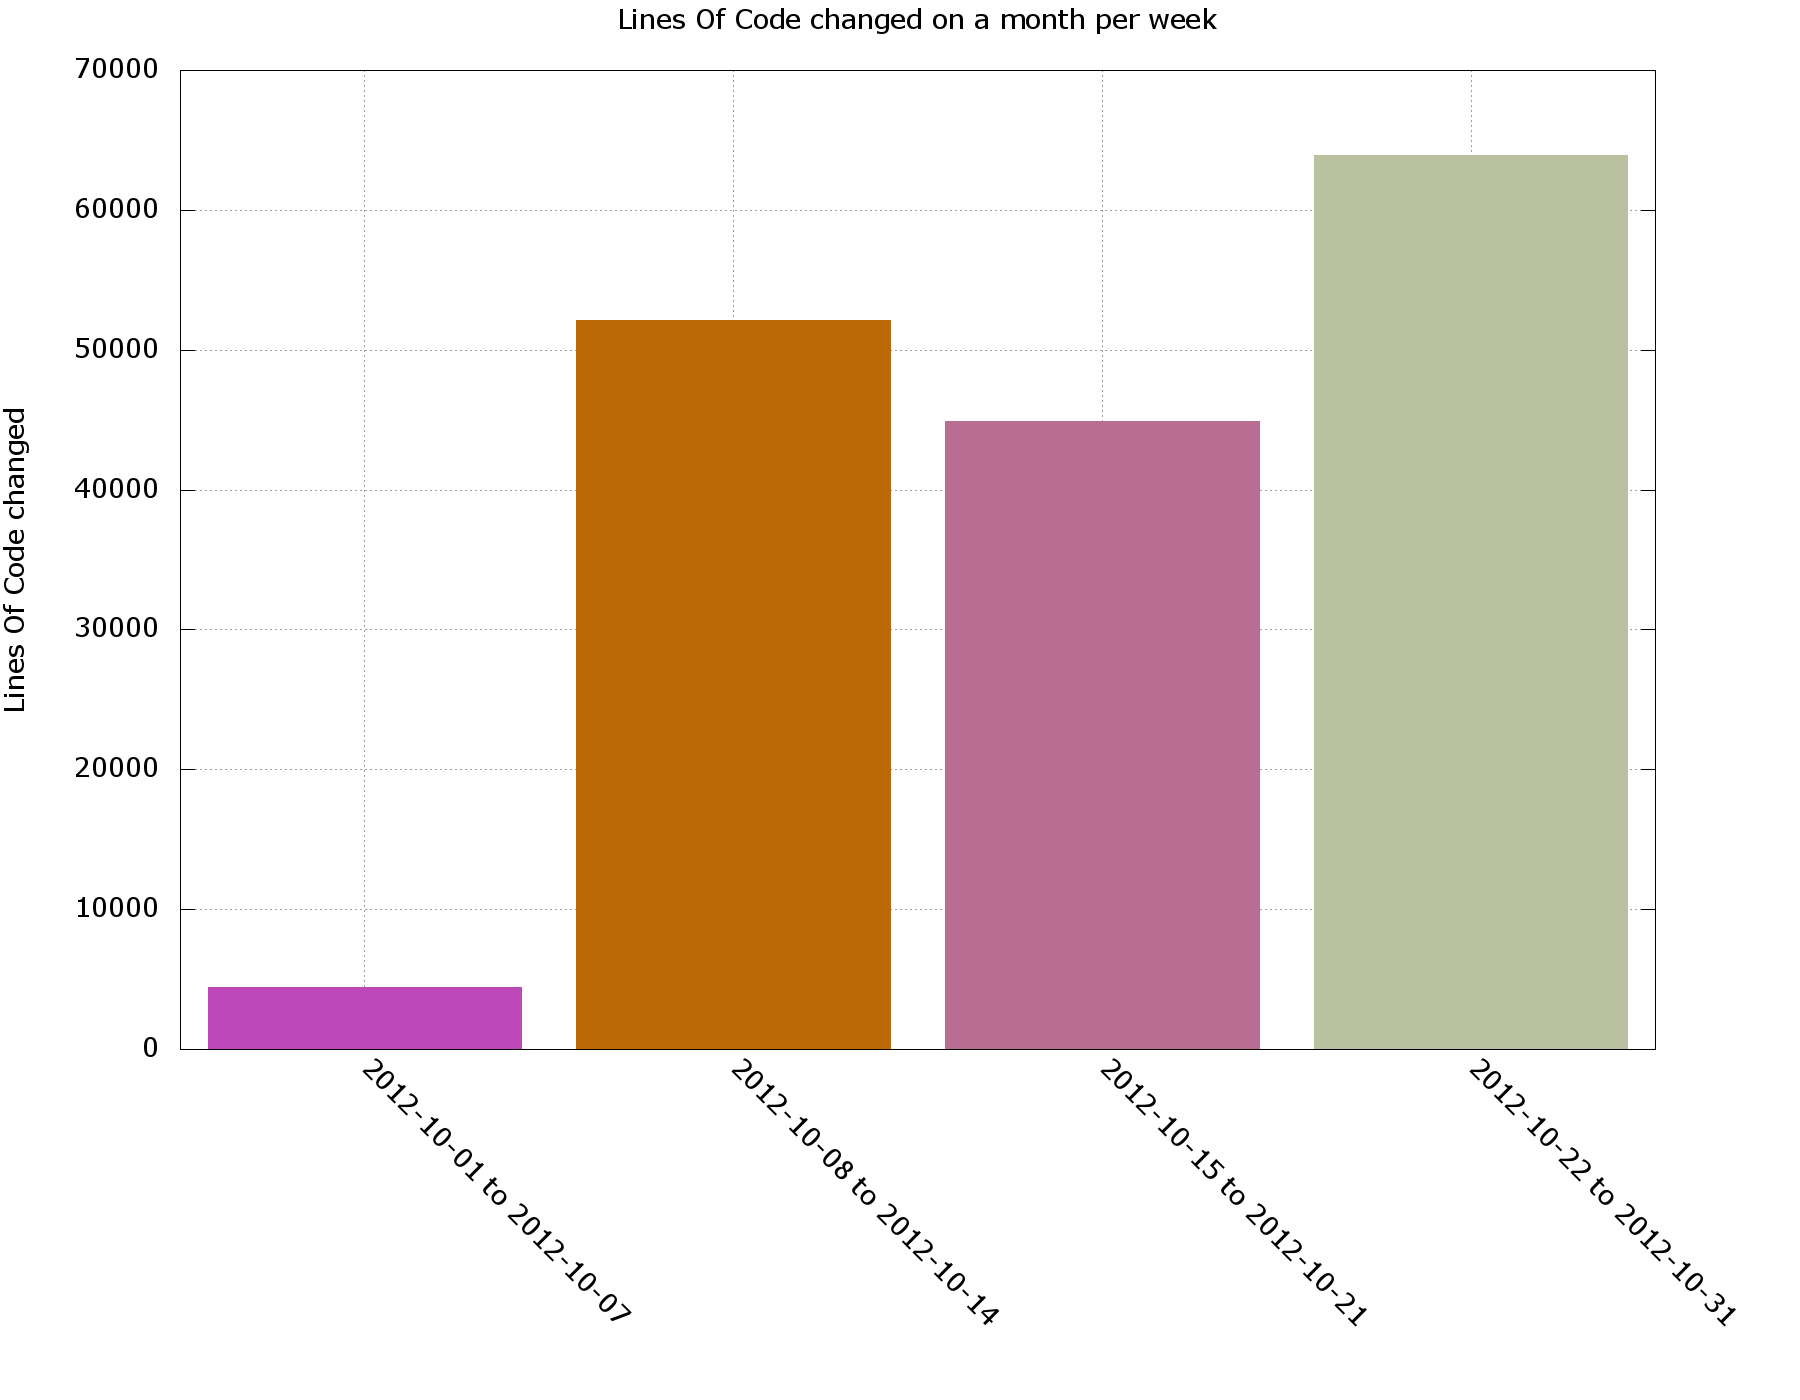
\includegraphics[width=\textwidth]{stats_monthweeks.png}
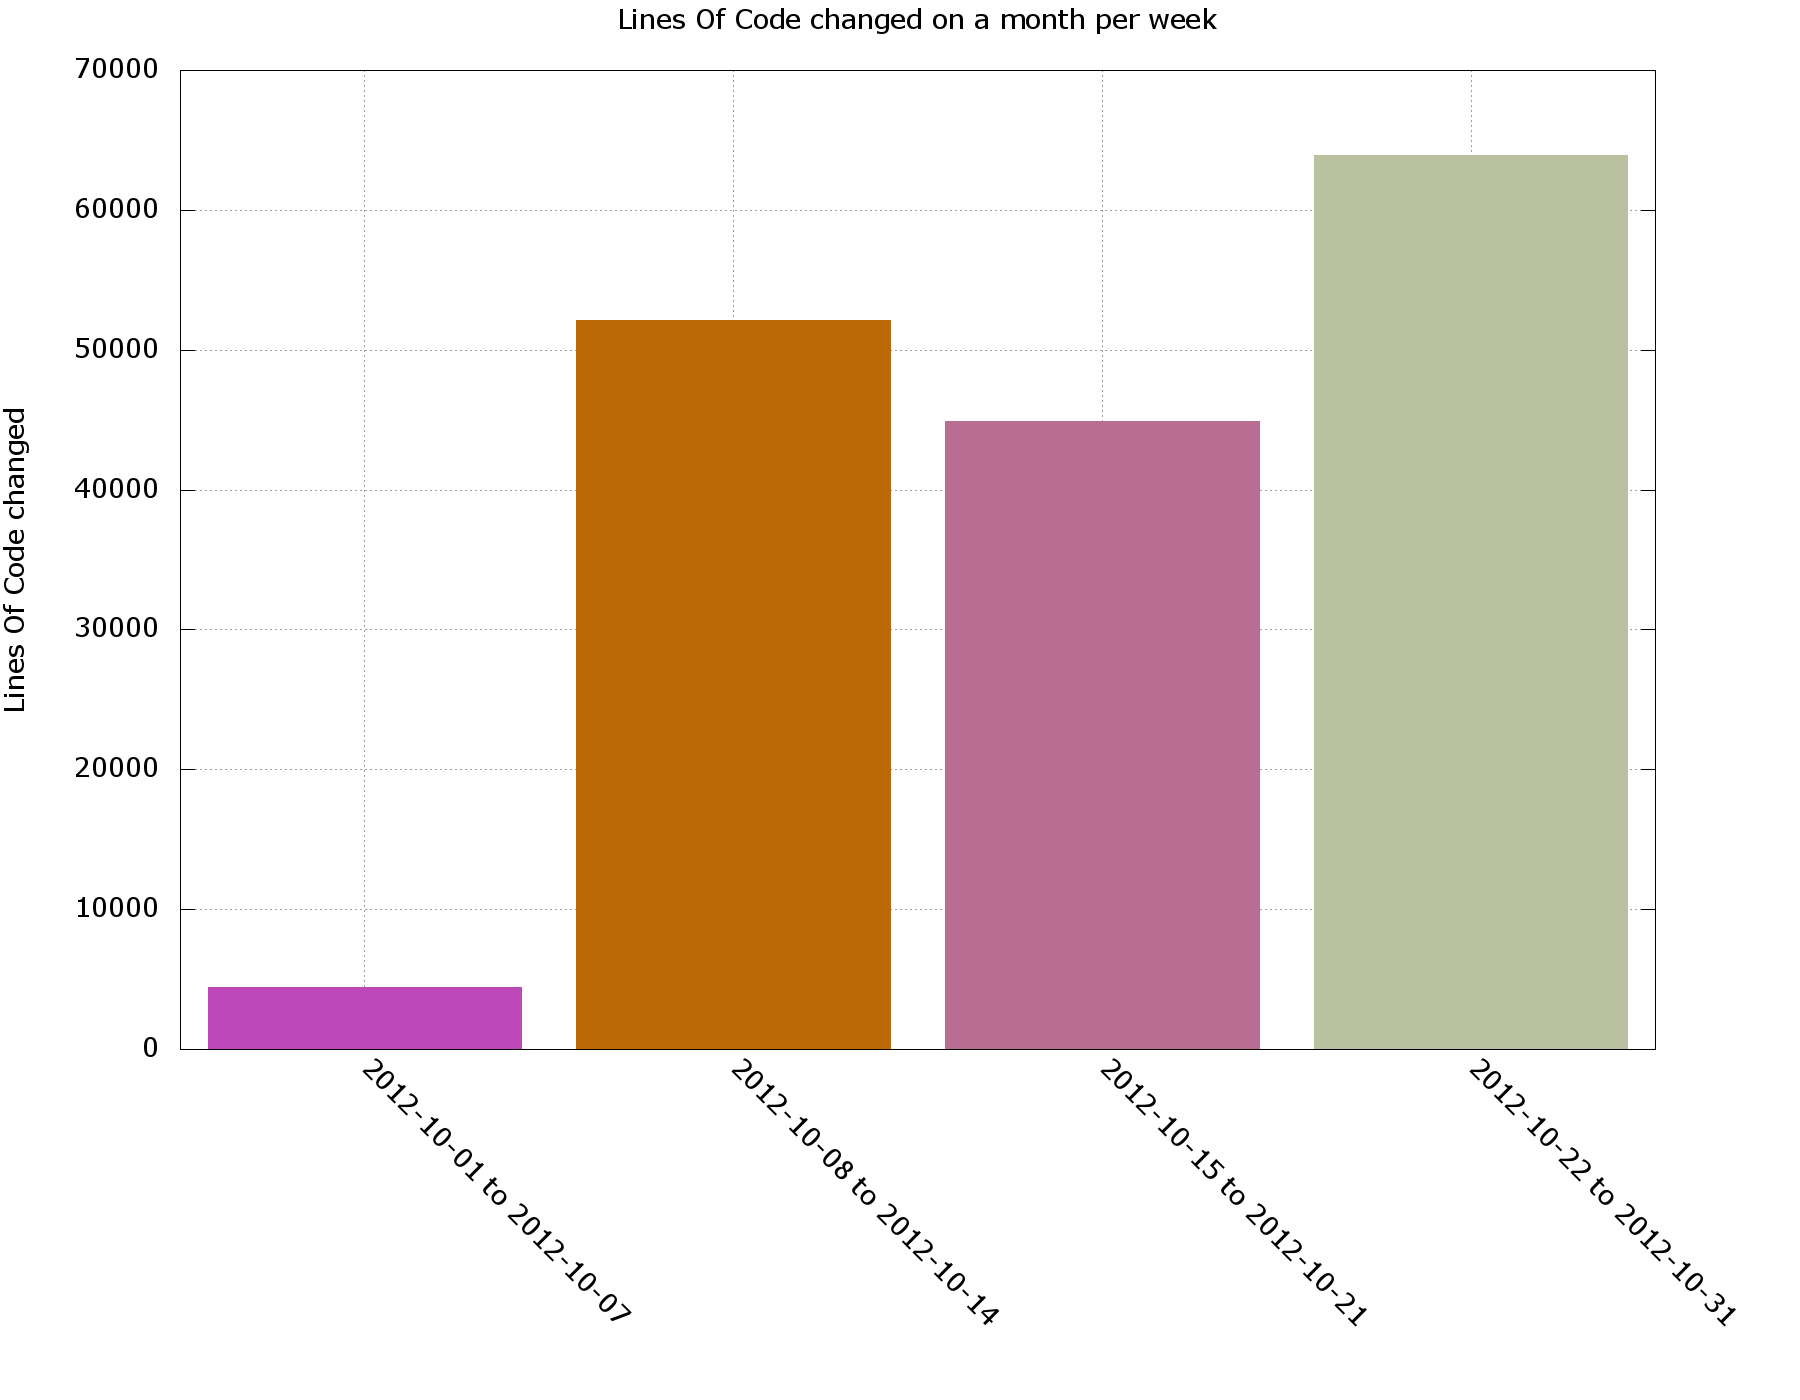
\includegraphics[scale=0.25]{stats_monthweeks.png}
The code for both python database application as well as bash scripts can be obtained on next link:\\
\\
\url{https://github.com/sarroutbi/MSWL_SUBJECTS/tree/master/PRACTICUM/plotter}\\
\\
\textbf{Time elapsed: 100 hours}

\section{Web Service prototype}
As an additional feature that could be included in Metrics Grimoire environment, a Web Service has been implemented. This prototype, implemented through gSoap framework, enables access from a external client to the statistics generated by Guilty, by parsing client's request, calling the plotter application described on previous chapter, parsing the plotting information and filling the response with the information obtained. The gSoap header file to implement the Web Service is described below:
\begin{verbatim}
//File: bikeGet.h
//gsoap ns2 service name: statsGet
//gsoap ns2 service namespace: urn: statsGet
//gsoap ns2 service location: http://sarroutbi.dyndns.org/statsGet.cgi

class guiltyStat
{
  char*  date;
  char*  file;
  char*  author;
  double loc;
};
int ns2__statsGet(char* date, char* file, char* author, guiltyStat \& stat);
\end{verbatim}
Besides the Web Service, a client has been implemented in order to show a way of how to connect and extract the statistics. This client, allows dumping the Lines Of Code of a certain date, enabling also filtering for a particular author and/or a particular file.\\
\\
The code for both Web Service as well as client, together with the .wsdl file of the Web Service, can be obtained on next link:\\
\\
\url{https://github.com/sarroutbi/MSWL_SUBJECTS/tree/master/PRACTICUM/ws/src/webservice/src}\\
\\
\textbf{Time elapsed: 75 hours}
\end{document}
